\documentclass[%
	11pt,
	a4paper,
	utf8,
	%twocolumn
		]{article}	

\usepackage{style_packages/podvoyskiy_article_extended}


\begin{document}
\title{Сборник задач с решениями по прикладной математике}

\author{\itshape Подвойский А.О.}

\date{}
\maketitle

\thispagestyle{fancy}

%Здесь приводятся заметки по специальным вопросам теории оптимизации


%\shorttableofcontents{Краткое содержание}{1}

\tableofcontents

\section{Комбинаторика}

\subsection{Основные соотношения}

Множество объектов предполагается гетерогенным, т.е. состоящим из \underline{\itshape различных} объектов (или объектов, считающихся в контексте рассматриваемой задачи различными)

\emph{Перестановка} Типичная смысловая нагрузка: <<Сколькими способами можно переставить $ n $ объектов?>>

$$ P_n = n! $$

\emph{Сочетание} Типичная смысловая нагрузка: <<Сколькими способами можно выбрать $ k $ объектов из $ n $?>> В сочетаниях порядок следования элементов в комбинации не имеет никакого значения

$$ C_n^k = \dfrac{n!}{k! \, (n-k)!} $$

\emph{Размещение} Типичная смысловая нагрузка: <<Сколькими способами можно выбрать $ k $ объектов (из $ n $) и \emph{в каждой выборке} переставить их местами (либо распределить между ними какие-нибудь уникальные атрибуты)?>> Размещения учитывают порядок следования элементов в комбинации

$$ A_n^k = C_n^k \, P_k $$

\emph{Перестановка с повторением} Типичная смысловая нагрузка: <<Количество способов, которыми можно переставить $ n $ объектов, среди которых 1-ый объект повторяется $ n_1 $ раз, 2-ой объект -- $ n_2 $ и т.д.?>>

$$ \stackrel{\circlearrowright}{P}_n = \dfrac{n!}{n_1! \, n_2 \, \ldots n_k}, \ \sum_{i=1}^k = n_i = 1 $$

\emph{Сочетания с повторениями} Типичная смысловая нагрузка: <<Для выбора предложено $ n $ множеств, каждое из которых состоит из одинаковых объектов. Сколькими способами можно выбрать $ k $ объектов?>>

$$ \stackrel{\circlearrowright}{C_n^k} = C_{n + k - 1}^k $$

\emph{Размещение с повторением} Типичная смысловая нагрузка: <<Сколько комбинаций можно построить из $ k $ объектов, каждый из которых может находиться в $ n $ состояниях?>>

$$ \stackrel{\circlearrowright}{A_n^k} = n^k $$

Число способов размещения $ n $ \emph{одинаковых} предметов по $ m $ \emph{различным} ящикам. Здесь важно имееть в виду, что некоторые ящики могут остаться пустыми
\begin{align*}
	\bar{C}_m^n = C_{m+n-1}^n = C_{m+n-1}^{m-1}
\end{align*}

Число способов размещения $ n $ \emph{одинаковых} объектов по $ m $ \emph{различным} ящикам при условии, что в каждом ящике должно быть не менее $ r $ объектов
\begin{align*}
	C^{m-1}_{n - m(r-1) -1}
\end{align*}

\textbf{Пример} \cite[\strbook{91}]{vilenkin:comb-2022} Сколькими способами могут распределяться 15 перенумерованных бильярдных шаров в 6 лузах?

Если каждый бильярдный шар рассматривать как объект с набором состояний <<попасть в первую лузу>>, <<попасть во вторую лузу>> и т.д., то число способов размещения $ n $ \emph{\underline{различных}} предметов по $ m $ \emph{\underline{различным}} ящикам можно найти по формуле размещения с повторениями, т.е. $ \stackrel{\circlearrowright}{A_{6}^{15}} = 6^{15} $. Здесь важно имееть в виду, что размещение с повторениями учитывает варианты, в которых все объекты (бильярдные шары) могут попасть в одну и ту же лузу, например, первый шар попал в 3-ью лузу, и второй шар попал в 3-ью лузу и т.д.

\textbf{Пример} \cite[\strbook{91}]{vilenkin:comb-2022} Трое ребят собрали с яблони 40 яблок. Сколькими способами они могут их разделить, если все яблоки считаются одинаковыми?

Здесь размещаемые предметы одинаковы -- нас интересует лишь, сколько яблок получит каждый, но не то, какие именно яблоки ему достанутся, т.е. способ раздела задается тройкой чисел (сколько яблок получит первый, второй, третий). Для решения этой задачи поступим так: добавим к собранным яблокам еще 2 одинаковые груши, а потом переставим всеми возможными способами 40 яблок и 2 груши. По формуле для перестановок с повторениями число таких перестановок равно $ 42! / (40! \, 2!) = 861 $.

Но каждой перестановке соответствует свой способ раздела яблок. Первому из ребят мы даем все яблоки, начиная от первого и до первой груши, второму -- все яблоки, попавшие между первой и второй грушей, а третьему -- все яблоки, лежащие после второй груши. Ясно, что при этом различным перестановкам соответствуют разные способы раздела. Таким образом, общее число способов раздела 861. При этом может случиться так, что одному (или даже двоим) участникам раздела ничего не достанется. Например, если одна из груш попадет при перестановке в начало, то лишается яблок первый из ребят, а если в конец -- то третий. Если же обе груши окажутся рядом, то ничего не получит второй. 

\vspace*{2mm}
\textbf{Пример} \cite[\strbook{610}]{shiryaev:prob-2013} Пусть $ \mathbf{A} = \{a_1, a_2, a_3, a_4\} $, $ | \mathbf{A} | = 4 $, $ n = 2 $.

\begin{itemize}
	\item Размещение без повторений $ A_4^2 = C_4^2 \, 2! = 12 $. 
	
	Соответствующие 12 \emph{\underline{упорядоченных}} (т.е. порядок следования элементов в выборке имеет значение!) выборок суть
	\begin{align*}
		(a_1, a_2), (a_1, a_3), (a_1, a_4), (a_2, a_1), (a_2, a_3), (a_2, a_4),\\ (a_3, a_1), (a_3, a_2), (a_3, a_4), (a_4, a_1), (a_4, a_2), (a_4, a_3)
	\end{align*}
    То есть \emph{размещение без повторений} в выборках учитывает порядок следования элементов и потому кортеж $ (a_1, a_2) $ и $ (a_2, a_1) $ это два разных кортежа! Так как <<без повторений>>, то среди рассмотренных выборок нет вариантов вида $ (a_i, a_i) $
    
    \item Сочетание без повторений $ C_4^2 = 6 $. Соответствующие 6 \emph{неупорядоченных} (порядок следования элементов не имеет значения!) выборок суть
    \begin{align*}
    	[a_1, a_2], [a_1, a_3], [a_1, a_4], [a_2, a_3], [a_2, a_4], [a_3, a_4]
    \end{align*} 
    \emph{Сочетание без повторений} в выборках не учитывает порядок следования элементов, поэтому кортежы $ [a_1, a_2] $ и $ [a_2, a_1] $ считаются эквивалентными. Так как <<без повторений>>, то в выборках нет вариантов вида $ [a_i, a_i] $
    
    \item Размещение с повторением $ 4^2 = 16 $. К 12 выборками $ A_4^2 $ добавляются еще выборки $ (a_1, a_1) $, $ (a_2, a_2) $, $ (a_3, a_3) $ и $ (a_4, a_4) $.
    
    \item Сочетание с повторением $ C_{4 + 2 -1}^2 = 10 $. К 6 выборкам $ C_4^2 $ добавляются еще выборки $ [a_1, a_1] $, $ [a_2, a_2]$, $ [a_3, a_3] $ и $ [a_4, a_4] $.
\end{itemize}




\subsection{Задача о комбинациях выхода пассажиров из лифта на разных этажах}

\paragraph{Постановка} В лифт 12-этажного дома сели 3 пассажира. Каждый независимо от других может выйти на любом (начиная со 2-ого) этаже. Сколькими способами пассажиры могут выйти из лифта?

\paragraph{Решение} Постановку задачи можно переформулировать по-другому. Сколько существует способов выйти 3 пассажирам на одном и том же этаже $ N_1 $ ИЛИ на двух разных этажах $ N_2 $ ИЛИ на трех разных этажах $ N_3 $?

Очевидно, что существует только 11 способов всем пассажирам выйти на одном и том же этаже, ведь $ N_1 = C_{11}^1 = 11 $.

С двумя этажами посложнее. Для начала следует понять сколько \emph{коммутативных\footnote{Потому что порядок следования номеров этажей не имеет никакого значения} 2-кортежей} из номеров этажей можно составить для 12-этажного здания. Другими словами, сколько существует способов выбрать 2 элемента из 11? Получается $ C_{11}^2 $ вариантов выбрать два разных номера этажа (например, 6-ой и 11-ый этажи). Для \emph{каждого} такого 2-кортежа нужно найти количество способов выбрать двух пассажиров из 3. То есть скольким числом способов 2 пассажира могут выйти на \emph{одном этаже}. Если пассажиров обозначить как $ x_1 $, $ x_2 $ и $ x_3 $, то получится, что можно составить $ C_3^2 $ \emph{уникальных} 2-кортежа $ (x_1, x_2) $, $ (x_2, x_3) $ и $ (x_1, x_3) $. Еще один очень важный момент заключается в том, что найденные 2-кортежи учитывают вариант, когда 2 пассажира выходят на каком-то одном этаже, например, на 6-ом, а третий пассажир на 11-ом. Но ведь нужно учесть симметрию для \emph{каждой} комбинации двух пассажиров, когда 2 пассажира выходят на 11-ом, а третий на 6-ом. То есть в данном случае требуется вычислить не сочетание, а размещение $ A_3^2 = C_3^2 \, P_2 $. Таким образом, пассажиры могут выйти на двух разных этажах $ N_2 = C_{11}^2 \, C_3^2 \, P_2 $ способами.

\remark{
Как вариант, вместо $ C_3^2 = 3 $ можно использовать $ C_3^1 = 3 $. То есть $ C_3^1 $ способами можно выбрать одного пассажира, а значит двух других 
}

Еще $ N_2 $ можно вычислить как $ C_3^2 \cdot 11 \cdot 10 $. Действительно, существует $ C_3^2 $ способа выбрать двух пассажиров, которые выйдут на одном этаже, и еще одного пассажира, который выйдет на другом. Но для \emph{каждой} такой комбинации можно рассматривать две уникальные группы пассажиров, одна группа пассажиров выходит на одном этаже, а другая -- на другом. Получается декартово произведение вариантов. Декартово произведение дублирует информацию и таким образом неявно учитывается перестановка номеров этажей.

Для трех этажей логика следующая. Скольким числом способов можно выбрать 3 разных номера этаже. То есть другими словами, сколько уникальных 3-кортежей (например, 5-ый этаж, 3-ий и 8-ой) можно составить из 11 вариантов. Очевидно, что $ C_{11}^3 $. Но для \emph{каждой} тройки этажей нужно еще рассмотреть перестановку пассажиров, ведь для 3-кортежа этажей (5, 3, 8) первый пассажир мог выйти на 5-ом этаже, второй -- на 3-ем, третий -- на 8-ом ИЛИ первый на 3-ем, второй -- на 5-ом и третий -- на 8-ом и т.д. То есть $ N_3 = C_{11}^3 P_3 $.

$ C_{11}^3 P_3 $ можно прочитать так: <<существует $ C_{11} ^3 $ выбрать 3 разных этажа и распределить по ним 3 пассажиров>>. То есть по сути это простое размещение.

И, наконец, существует $ N_1 + N_2 + N_3 $ спосбов выйти 3 пассажирам из лифта.

Проще эту задачу можно решить, если \emph{каждого} из 3 пассажиров рассматривать как некоторый объект, у которого есть несколько состояний -- состояние <<выйти на 1-ом этаже>>, состояние <<выйти на 2-ом этаже>> и т.д. Всего состояний 11. Тогда справедлива формула размещения с повторениями $ 11^{3} = 1331 $.

\subsection{Сочетания на двудольном графе}

\paragraph{Постановка} В студенческой группе 10 парней и 13 девченок. Сколькими способами можно составить разнополую пару?

\paragraph{Решение} Исходную постановку задачи можно переформулировать в терминах двудольных графов. Одна доля <<парни>>, другая -- <<девченки>>. Таким образом, нас интересует скольким числом способов можно связать \emph{каждый} элемент из одной доли \emph{с каждым} элементом из другой. Получается простое произведение
\begin{align*}
	C_{10}^1 \cdot C_{13}^1 = 10 \cdot 13 = 130.
\end{align*}

Прочитать $ C_{10}^1 \cdot C_{13}^1 $ можно как <<выбрать один элемент из одной доли \textbf{И} выбрать другой элемент из другой доли>>.

Если бы требовалось найти количество способов выбрать два элемента одного типа (например, выбрать двух человек одного пола) из двудольного графа, то нужно было бы сочетания складывать, т.е. $ C_{10}^2 + C_{13}^2 $. То есть читается так: <<выбрать два элемента из одной доли \textbf{ИЛИ} два элемента из другой>>.

\section{Теория вероятностей}

\subsection{Задача о вероятности сохранения не менее половины нейронов сети после процедуры прореживания}

\paragraph{Постановка} Задан многослойный персептрон с $ N $ нейронами. Найти вероятность события состоящего в том, что после процедуры прореживания (dropout) будет сохранено не менее половины нейронов.

\paragraph{Решение} Если каждый нейрон рассматривать как объект с бинарным состоянием (<<нейрон включен>>, <<нейрон выключен>>), то число всех возможных комбинаций \emph{с учетом порядка следования нейронов} можно найти с помощью размещения с повторением, а именно $ 2^N - 1 $. Здесь <<-1>>, потому что нужно отбросить вариант, когда все нейроны отключены. То есть $ | \Omega | =  2^N - 1 $ это количество всех возможных исходов.

Остается найти число благоприятствующих исходов и тогда с помощью классической частотной интерпретации можно будет найти искомую вероятность.

По условию задачи требуется найти вероятность сохранения не менее половины нейронов. Следовательно требуется рассмотреть варианты, когда нейронов остается (половина\footnote{С округлением вверх}) ИЛИ (половина + 1) ИЛИ (половина + 2) и т.д. То есть $ \sum\limits_{k=0}^{N - \lceil N / 2 \rceil} C_{N}^{ \lceil N/2 \rceil + k } $.

Тогда искомая вероятность будет
\begin{align*}
	\boxed{ \mathbf{P} (X \geqslant \lceil N / 2 \rceil ) = \dfrac{1}{2^N - 1} \sum\limits_{k=0}^{N - \lceil N / 2 \rceil} C_N^{ \lceil N / 2 \rceil + k} }
\end{align*}

\subsection{Задача о случайном выборе двух натуральных чисел из конечной последовательности}

\paragraph{Постановка} Даны натуральные числа $ m $ и $ n $, причем $ m < n $. Из чисел $ 1, 2, \ldots, n $ последовательно выбирают наугад два различных числа. Найдите вероятность того, что разность между первым выбранным числом и вторым будет не меньше $ m $.

\paragraph{Решение} Представляется удобным задачу переформулировать следующим образом. При натуральных $ m $ и $ n $ ($ m < n $) найти вероятность события, состоящего в том, что второе случайно выбранное из последовательности $ \{1, 2, \ldots, n \} $ число $ d_2 $, окажется не больше первого случайно выбранного из той же последовательности числа $ d_1 $, уменьшенного на $ m $.

По условию задачи
\begin{align}\label{eq:d1d2}
	d_2 \leqslant d_1 - m 
\end{align}

Из неравенства \eqref{eq:d1d2} следует, что $ m < d_1 $, так как в противном случае число $ d_2 $ не будет принадлежать множеству натуральных чисел, т.е. $ d_2 \notin \mathbb{N}_{> 0} $.

Предполагается, что в задаче речь идет о множестве натуральных чисел, \emph{не} расширенном нулем. Но даже если бы множество было расширено нулем $ \mathbb{N} \cup \{0\} $, то при $ m = 0 $ для числа $ d_2 $ нарушились бы условия задачи, ведь $ d_2 \in \{ 1, 2, \ldots, n \}$ . Действительно, если $ m = 0 $, то $ d_2 < d_1 $ (случай равенства чисел исключен, так как по условию задачи $ d_1 \neq d_2 $). И тогда при $ d_1 = 1 $ переменная $ d_2 $ может принимать только \emph{неположительные} значения, что противоречит условию задачи.

Правой границей для $ d_1 $ будет $ d_1^r = n $, т.е. $ m < d_1 \leqslant n $. Для того чтобы число $ d_2 $ не нарушало границы множества натуральных чисел и одновременно выполнялось условие \eqref{eq:d1d2} левая граница числа $ d_1 $ должна быть $ d_1^l = m + 1, \ m \in \mathbb{N}_{> 0} $.

В итоге $ 1 \leqslant m < d_1 \leqslant n \ \rightarrow \ m + 1 \leqslant d_1 \leqslant n $.

Таким образом, требуется найти вероятность выполнения ограничения \eqref{eq:d1d2}, используя формулу полной вероятности
\begin{align}\label{eq:pd1d2}
	\mathbf{P}(d_2 \leqslant d_1 - m) = \sum_{d_1 = m + 1}^{n} \mathbf{P}(\check{d_2} \leftarrow \check{d}_1) \, \mathbf{P}(\check{d_1}),
\end{align}
где $ \mathbf{P}(\check{d_2} \leftarrow \check{d}_1) $ -- вероятность выбора числа $ d_2 $ таким способом, чтобы не нарушить ограничение~\eqref{eq:d1d2} при выбранном числе $ d_1 $, $ \mathbf{P}(\check{d_1}) $ -- вероятность выбора числа $ d_1 $.

Вероятность выбора первого числа $ d_1 $ определяется как
\begin{align*}
	\mathbf{P}(\check{d_1}) = \dfrac{1}{n}
\end{align*}

\remark{
	Несложно впасть в искушение определить вероятность $ \mathbf{P}(\check{d_1}) $ как $ (n - m) / n $, потому что кажется, что $ d_1 $ может принимать только значения большие $ m + 1 $ и меньшие $ n $, однако это неверно, так как в качестве первого числа $ d_1 $ можно выбрать любое число от 1 до $ n $, а ограничения для $ d_1 $ учитываются с помощью верхнего и нижнего предела суммы формулы полной вероятности
}

Вероятность выбора второго числа $ d_2 $ при соблюдении ограничения \eqref{eq:d1d2} можно записать следующим образом
\begin{align*}
	\mathbf{P}(\check{d_2} \leftarrow \check{d}_1) = \dfrac{d_1 - m}{n - 1}
\end{align*}

Знаменатель $ n - 1 $ учитывает, что число $ d_1 $ выбрано на первом шаге.

Теперь формулу \eqref{eq:pd1d2} можно переписать
\begin{align*}
	\mathbf{P}(d_2 \leqslant d_1 - m) = \sum_{d_1 = m + 1}^n \dfrac{d_1 - m}{n - 1} \cdot \dfrac{1}{n} = \dfrac{1}{n} \sum_{d_1 = m + 1}^n \dfrac{d_1 - m}{n - 1} = \dfrac{1}{n (n-1)} \sum_{k=1}^n k 
\end{align*}

Сумма в последнем соотношении очевидно представляет собой арифметическую прогрессию с первым элементом $ a_1 = 1 $, разностью $ d = 1 $, длинной $ n' = n - (m + 1) + 1 = n - m $ и суммой $ n' $ элементов $ S_{n'} = \dfrac{2 a_1 + d (n' - 1)}{2} n' $. То есть $ \sum\limits_{k=1}^{n - m} k = \dfrac{(n - m + 1)(n - m)}{2} $.

Тогда искомая вероятность

\begin{align}\label{eq:pd2leqd1}
	\boxed{\mathbf{P}(d_2 \leqslant d_1 - m) = \dfrac{(n - m + 1)(n - m)}{2n(n-1)}}
\end{align}


На \pic{fig:kde_d2_leq_d1_minus_m} приведено распределение вероятности выполнения ограничения \eqref{eq:d1d2} при различных значениях длины последовательности $ n $ и смещении $ m $.

Любопытно,
\begin{itemize}
	\item что при $ m = 1 $ вероятность $ \mathbf{P}(d_2 \leqslant d_1 - m) = 1/2 $, не зависимо от длины последовательности,
	
	\item чем длинее последовательность, тем ближе вероятность $ \mathbf{P}(d_2 \leqslant d_1 - m) $ к $ 1/2 $, не зависимо от $ m $.
\end{itemize}

\begin{figure}[!h]
	\centering
	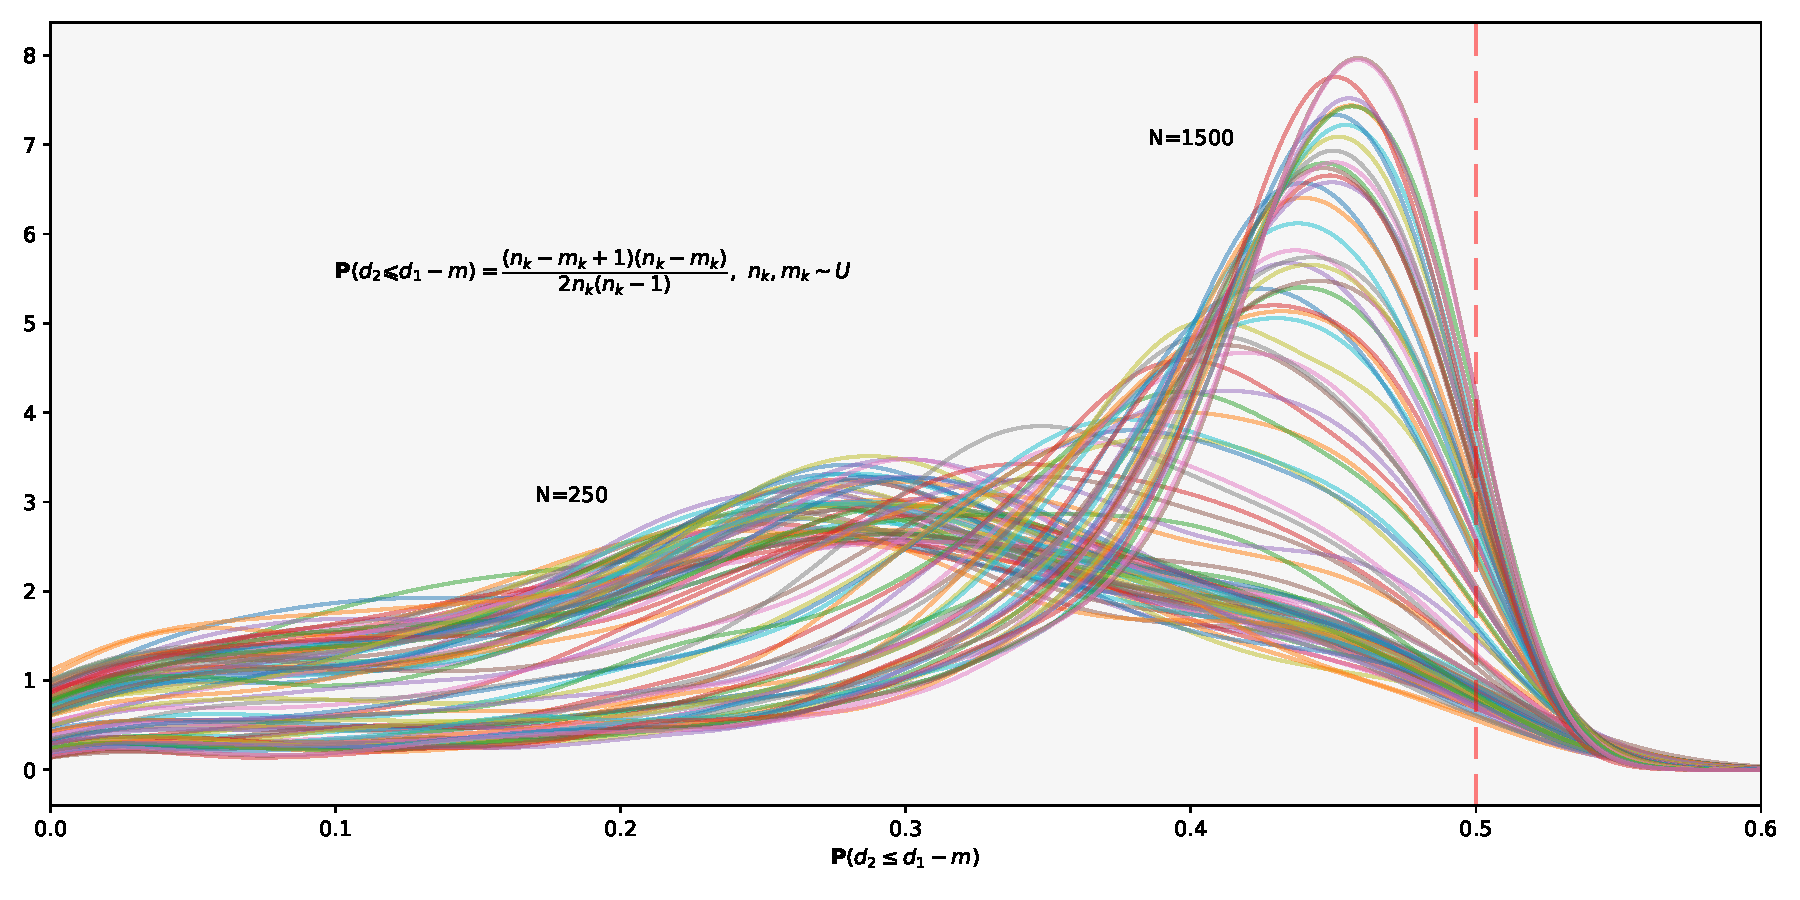
\includegraphics[scale=0.5]{figures/kde_d2_leq_d1_minus_m.pdf}
	\caption{ Распределение вероятности $ \mathbf{P}(d_2 \leqslant d_1 - m) $ в зависимости от различных значений длины последовательности $ n $ и смещения $ m $ }\label{fig:kde_d2_leq_d1_minus_m}
\end{figure}

\subsection{Задача о математическом ожидании числа остановок лифта}

\paragraph{Постановка} На первом этаже одиннадцатиэтажного дома в лифт зашли четверо человек. Будем считать, что каждый пассажир лифта независимо и случайно выбирает этаж, на который ему надо добраться. Найти математическое ожидание числа остановок лифта (лифт останавливается только на этажах, выбранных пассажирами, на остановках новые люди в лифт не входят).

\paragraph{Решение} Очевидно, что максимальное число остановок лифта для четырех пассажиров $ N_{\max} = 4 $. Число остановок лифта $ N $ это дискретная случайная величина, математическое ожидание которой для четырех этажей определяется как
\begin{align}\label{eq:expct}
	\mathbf{E}[N] = \sum_{k=1}^{N_{max}} k \, p_k
\end{align}

Учитывая, что события <<Одна остановка лифта>>, <<Две остановки лифта>> и пр. образуют полную группу, т.е. $ \sum p_k = 1 $, соотношение \eqref{eq:expct} можно упростить
\begin{align*}
	\mathbf{E}[N] = (1 - p_2 - p_3 - p_4) + 2 p_2 + 3 p_3 + 4 p_4 = 1 + p_2 + 2 p_3 + 3 p_4
\end{align*}

Теперь можно приступать к вычислению вероятности события, состоящего в том, что лифт сделает 2 остановки, 3 остановки и т.д. Кажется логичным, использовать частотную интерпретацию вероятности.

Если каждого пассажира рассматривать как объект с 10-ью состояниями (<<выйти на 2-ом этаже>>, <<выйти на 3-ем этаже>> и т.д.), то с помощью формулы \emph{размещения с повторением}, можно найти число всех возможных исходов, а именно $ \stackrel{\circlearrowright}{A_{10}^4} = 10^4 $.

Для того чтобы, найти число способов, которым 4 пассажира могут выйти из лифта на 2 разных этажах, сначала нужно найти число способов выбрать 2 разных этажа из 10 вариантов. Это очевидно простое сочетание $ C_{10}^2 $. Другими словами, существует $ C_{10}^2 $ способов составить коллекцию \emph{неупорядоченных} 2-коретежей: (3,5), (5,11) и т.д. \emph{Для каждого} варианта из $ C_{10}^2 $ существует несколько схем выхода пассажиров.

Для примера рассмотрим кортеж (5,11) и схему <<$ 1 | 3 $>>, когда один пассажир $ \{x_j\}_{j=1}^4 $ выходит на каком-то одном этаже (например, на 5-ом), а трое других -- на каком-то другом этаже (т.е. в данном случае на 11-ом)
\begin{align*}
	\begin{matrix}
		x_1 & x_2 & x_3 & x_4 \\
		\bullet & \cdot & \cdot & \cdot \\
		\cdot & \bullet & \cdot & \cdot \\
		\cdot & \cdot & \bullet & \cdot \\
		\cdot & \cdot & \cdot & \bullet 
	\end{matrix}
\end{align*}

Для наглядности выпишем получившиеся схемы для случая, когда пассажир-одиночка выходит на 5-ом этаже
\begin{align*}
	x_1 \rightarrow 5, (x_2, x_3, x_4) \rightarrow 11\\
	x_2 \rightarrow 5, (x_1, x_3, x_4) \rightarrow 11\\
	x_3 \rightarrow 5, (x_1, x_2, x_4) \rightarrow 11\\
	x_4 \rightarrow 5, (x_1, x_2, x_3) \rightarrow 11
\end{align*}

Может показаться, что эти схемы описывают все варианты выхода пассажиров на двух разных этажах. Но ведь пассажир-одиночка мог выйти и на 11 этаже (а не на 5-ом как в приведенных схемах). А так как нас интересуют \emph{все} благоприятствующие исходы, то при подсчете вариантов выхода необходимо учесть симметрию
\begin{align*}
	\begin{matrix}
		x_1 \rightarrow 11, (x_2, x_3, x_4) \rightarrow 5\\
		x_2 \rightarrow 11, (x_1, x_3, x_4) \rightarrow 5\\
		x_3 \rightarrow 11, (x_1, x_2, x_4) \rightarrow 5\\
		x_4 \rightarrow 11, (x_1, x_2, x_3) \rightarrow 5
	\end{matrix}
\end{align*}

Таким образом, для схемы <<$ 1|3 $>> существует $ C_{10}^2 \cdot C_4^1 \cdot 2! $ вариантов выхода. Перейдем к рассмотрению схемы <<$ 2 | 2 $>>, когда какие-то два пассажира выходят на каком-то одном этаже, а остальные -- на каком-то другом, т.е.
\begin{align*}
	\begin{matrix}
		x_1 & x_2 & x_3 & x_4 \\
		\bullet & \bullet & \cdot & \cdot \\
		\cdot & \bullet & \bullet & \cdot \\
		\cdot & \cdot & \bullet & \bullet \\
		\bullet & \cdot & \bullet & \cdot \\
		\cdot & \bullet & \cdot & \bullet \\
		\bullet & \cdot & \cdot & \bullet \\
	\end{matrix}
\end{align*}

Снова для наглядности выпишем получившиеся схемы
\begin{align*}
	(x_1, x_2) \rightarrow 5, (x_3, x_4) \rightarrow 11 \\
	(x_2, x_3) \rightarrow 5, (x_1, x_4) \rightarrow 11 \\
	(x_3, x_4) \rightarrow 5, (x_1, x_2) \rightarrow 11 \\
	(x_1, x_3) \rightarrow 5, (x_2, x_4) \rightarrow 11 \\
	(x_2, x_4) \rightarrow 5, (x_1, x_3) \rightarrow 11 \\
	(x_1, x_4) \rightarrow 5, (x_2, x_3) \rightarrow 11
\end{align*}

И еще выпишим, как в предыдущем случае, схемы с учетом симмертрии
\begin{align*}
	\begin{matrix}
		(x_1, x_2) \rightarrow 11, (x_3, x_4) \rightarrow 5 \\
		(x_2, x_3) \rightarrow 11, (x_1, x_4) \rightarrow 5 \\
		(x_3, x_4) \rightarrow 11, (x_1, x_2) \rightarrow 5 \\
		(x_1, x_3) \rightarrow 11, (x_2, x_4) \rightarrow 5 \\
		(x_2, x_4) \rightarrow 11, (x_1, x_3) \rightarrow 5 \\
		(x_1, x_4) \rightarrow 11, (x_2, x_3) \rightarrow 5
	\end{matrix}
\end{align*}

Несложно заметить, что схемы второй группы дублируют информацию. Например, 3-ья сверху схема второй группы $ (x_3, x_4) \rightarrow 11, (x_1, x_2) \rightarrow 5 $ это тоже самое, что и первая схема первой группы $ (x_1, x_2) \rightarrow 5, (x_3, x_4) \rightarrow 11 $. Таким образом, для схемы <<$ 2|2 $>> существует $ C_{10}^2 \cdot C_4^2 $ способов выйти на двух разных этажах.

Тогда вероятность двух остановок лифта может быть вычислена как
\begin{align*}
	p_2 = \mathbf{P}(N = 2) = \dfrac{ C_{10}^2 \cdot (2! \cdot C_4^1 + C_4^2)}{ 10^4 } = 0.063
\end{align*}

Аналогично для трех остановок лифта сначала найдем количество способов выбрать 3 этажа из 10, то есть $ C_{10}^3 $. \emph{Для каждого} 3-кортежа  из коллекции длины $ C_{10}^3 $ существует несколько схем выхода пассажиров (приведены первые три схемы)
\begin{align*}
	\begin{matrix}
		x_1 & x_2 & x_3 & x_4 \\
		\cdot & \ast & \bullet & \bullet \\
		\cdot & \bullet & \ast & \bullet \\
		\cdot & \bullet & \bullet & \ast \\
		... & {} & {} & {}
	\end{matrix}
\end{align*}

Количество схем можно найти по формуле \emph{перестановки с повторениями}, т.е. $ \stackrel{\circlearrowright}{P}{}_4^{(1,1,2)} = 12 $ или с помощью комбинаторного произведения $ C_4^2 \cdot C_2^1 = 12 $.

Для примера, рассмотрим, 3-кортеж (3,8,11). Пусть в первой строке первого столбца $ (x_3, x_4) = 11 $, второго -- $ (x_3, x_4) = 8 $ и третьего -- $ (x_3, x_4) = 3 $, тогда получим следующие варианты
\begin{align*}
	\begin{matrix}
		{} & x_1 & x_2 & x_3 & x_4 \\
		{\color{blue}1} & 3 & 8 & 11 & 11 \\
		{\color{blue}2} & 3 & 11 & 8 & 11 \\
		{\color{blue}3} & 3 & 11 & 11 & 8 \\
		{\color{blue}4} & 8 & 3 & 11 & 11 \\
		{\color{blue}5} & 8 & 11 & 3 & 11 \\
		{\color{blue}6} & 8 & 11 & 11 & 3 \\
		{\color{blue}7} & 11 & 3 & 8 & 11 \\
		{\color{blue}8} & 11 &  3 & 11 & 8 \\
		{\color{blue}9} & 11 & 8 & 3 & 11 \\
		{\color{blue}10} & 11 & 8 & 11 & 3 \\
		{\color{blue}11} & 11 & 11 & 3 & 8 \\
		{\color{blue}12} & 11 & 11 & 8 & 3
	\end{matrix}
    \qquad
	\begin{matrix}
		x_1 & x_2 & x_3 & x_4 \\
		3 & 11 & 8 & 8 \\
		3 & 8 & 11 & 8 \\
		3 & 8 & 8 &11 \\
		11 & 3 & 8 & 8 \\
		11 & 8 & 3 & 8 \\
		11 & 8 & 8 & 3 \\
		8 & 3 & 11 & 8 \\
		8 & 3 & 8 & 11 \\
		8 & 11 & 3 & 8 \\
		8 & 11 & 8 & 3 \\
		8 & 8 & 3 & 11 \\
		8 & 8 & 11 & 3 \\
	\end{matrix}
    \qquad
    \begin{matrix}
    	x_1 & x_2 & x_3 & x_4 \\
    	8 & 11 & 3 & 3 \\
    	8 & 3 & 11 & 3 \\
    	8 & 3 & 3 & 11 \\
    	11 & 8 & 3 & 3 \\
    	11 & 3 & 8 & 3 \\
    	11 & 3 & 3 & 8 \\
    	3 & 8 & 11 & 3 \\
    	3 & 8 & 3 & 11 \\
    	3 & 11 & 8 & 3 \\
    	3 & 11 & 3 & 8 \\
    	3 & 3 & 8 & 11 \\
    	3 & 3 & 11 & 8
    \end{matrix}
\end{align*}

Таким образом, вероятность трех остановок
\begin{align*}
	p_3 = \mathbf{P}(N = 3) = \dfrac{ C_{10}^3 \cdot \stackrel{\circlearrowright}{P}{}_4^{(1,1,2)} \cdot 3 }{ 10^4 } = 0.432
\end{align*}



И, наконец, для четырех этажей сначало нужно найти количество способов выбрать 4 этажа из 10, т.е. $ C_{10}^4 $ и учесть распределение 4 этажей между 4 пассажирами, т.е. $ C_{10}^4 \cdot 4! $

Тогда вероятность четырех остановок
\begin{align*}
	p_4 = \mathbf{P}(N = 4) = \dfrac{ C_{10}^4 \cdot 4! }{ 10^4 } = 0.504
\end{align*}

Принимая во внимание, что вероятность выхода всех пассажиров на одном и тоже этаже $ C_{10}^1 \cdot C_4^4 / 10^4 = 0.001 $, проверим условие полной группы
\begin{align*}
	\sum_{k}^{N_{\max}} p_k = 0.001 + 0.063 + 0.432 + 0.504 = 1
\end{align*}

Искомое математическое ожидание числа остановок составит
\begin{align*}
	\boxed{\mathbf{E}[N] = 1 \cdot 0.001 + 2 \cdot 0.063 + 3 \cdot 0.432 + 4 \cdot 0.504 = 3.439}
\end{align*}

Более корткое решение можно получить \emph{методом индикаторов}.

Введем
\begin{itemize}
	\item бинарную дискретную случайную величину $ X_n, \, n = 2, \ldots, 11 $
	\begin{align*}
		X_n = \mathcal{I} \ (\text{<<остановка на $ n $-ом этаже>>})
	\end{align*}
	с вероятностями событий <<на $ n $-ом этаже была остановка>> $ \mathbf{P}(X_n = 1) $ и <<на $ n $-ом этаже не было остановки>> $ \mathbf{P}(X_n = 0) $
	
	\item дискретную случайную величину $ \xi_n $ -- <<номер этажа, на котором живет $ k $-ый человек>>
\end{itemize}


По условию задачи 

\begin{align*}
	\mathbf{P}(\xi_k = 2) = \mathbf{P}(\xi_k = 3) = \ldots = \mathbf{P}(X_k = 11) = 1/10
\end{align*}

Математическое ожидание события <<на 2-ом этаже была остановка>> \emph{или} <<на 3-ем этаже была остановка>> \emph{или} и т.д. будет иметь вид
\begin{align*}
	N = \mathbf{E} (X_2 + X_3 + \ldots + X_{11}) = \sum_{k=2}^{11} \mathbf{E}(X_k)
\end{align*}

Математическое ожидание дискретной бинарной случайной величины $ X_n $ определяется как $ \mathbf{E}X_n = 0 \cdot \mathbf{P}(X_n = 0) + 1 \cdot \mathbf{P}(X_n = 1) $ для любого этажа $ n = 2, \ldots, 11 $. Очевидно, события $ X_n = 1 $ <<был выход на $ n $-ом этаже>> и $ X_n  = 0 $ <<не было выхода на $ n $-ом этаже>> образуют полную группу.

Тогда
\begin{align*}
	 \mathbf{P}(X_n = 1) = 1 - \mathbf{P}(X_n = 0)
\end{align*}

Событие $ X_n = 0 $ <<не было выхода на $ n $-ом этаже>> означает, что первый пассажир $ \xi_1 $ не вышел на $ n $-ом этаже \emph{и} второй пассажир не вышел на $ n $-ом этаже \emph{и} и т.д., т.е.
$$
\mathbf{P}(X_n = 0) = \mathbf{P}(\xi_1 \neq n, \xi_2 \neq n, \ldots, \xi_{10} \neq n)
$$ 
Так как события $ \xi_1 \neq n $, $ \xi_2 \neq n $ и т.д. независимые, то
\begin{align*}
	\mathbf{P}(X_n = 1) = 1 - \mathbf{P}(\xi_1 \neq n) \cdot \mathbf{P}(\xi_2 \neq n) \cdot \mathbf{P}(\xi_{3} \neq n) \cdot \mathbf{P}(\xi_{4} \neq n)
\end{align*}

Вероятность не выйти на $ n $-ом этаже $ \mathbf{P}(\xi_k \neq n) = 1 - 1 / 10 , \, \forall k$. Тогда
\begin{align*}
	\mathbf{P}(X_n = 1) = 1 - (9 / 10)^{4} = 0.3439
\end{align*}

И, наконец, искомое математическое ожидание
\begin{align*}
	\boxed{\sum_{k=2}^{11} \mathbf{E} X_k = \mathbf{P}(X_k) \cdot 10 = 3.439}
\end{align*}

\subsection{Задача о математическом ожидании числа <<успехов>> в бесконечной бинарной последовательности}

\paragraph{Постановка} Организаторы выпускного тестирования на одном из курсов решили опробовать новый формат: тестирование длится до тех пор, пока сдающий либо два раза подряд неверно ответит на вопросы, либо пока он не ответит два раза подряд верно (т.е. теоретически, тестирование может длиться бесконечно долго, если сдающий отвечает верно ровно через раз). Найдите математическое ожидание числа вопросов, на которые ответит сдающий, если он на них отвечает неверно с вероятностью $ p = 1/3 $.

\paragraph{Решение}

Число ответов $ N $ это, очевидно, дискретная случайная величина. Через $ p_k $ обозначим вероятность, что сдающий даст $ k $ верных ответов. Тогда математическое ожидание будет
\begin{align*}
	\mathbf{E}N = \sum_{k=0}^{\infty} k \, p_k
\end{align*}

Рассмотрим несколько первых последовательностей
\begin{align*}
\begin{matrix}
\times & \times & (0) \\
\times & \bullet & \bullet & (2) \\
\times & \bullet & \times & \times & (1) \\
\times & \bullet & \times & \bullet & \bullet & (3) \\
\times & \bullet & \times & \bullet & \times & \times & (2) \\
\times & \bullet & \times & \bullet & \times & \bullet & \bullet & (4) \\
\times & \bullet & \times & \bullet & \times & \bullet & \times & \times & (3) \\
\times & \bullet & \times & \bullet & \times & \bullet & \times & \bullet & \bullet & (5) \\
\ldots
\end{matrix}
\hspace*{5mm}
\begin{matrix}
	\bullet & \bullet & (2) \\
	\bullet & \times & \times & (1) \\
	\bullet & \times & \bullet & \bullet & (3) \\
	\bullet & \times & \bullet & \times & \times & (2) \\
	\bullet & \times & \bullet & \times & \bullet & \bullet & (4) \\
	\bullet & \times & \bullet & \times & \bullet & \times & \times & (3) \\
	\bullet & \times & \bullet & \times & \bullet & \times & \bullet & \bullet & (5) \\
	\bullet & \times & \bullet & \times & \bullet & \times & \bullet & \times & \times & (4) \\
	\ldots
\end{matrix}
\end{align*}

Пусть $ p $ -- это вероятность дать верный ответ, а $ q $ -- это вероятность дать неверный ответ. Тогда вероятность, что сдающий
\begin{itemize}
	\item даст 0 верных ответов: $ q^2 p^0 $,
	
	\item даст 1 верный ответа: $ \underbrace{p \, q^3}\limits_{\times} + \underbrace{p \, q^2}\limits_{\bullet} $,
	
	\item даст 2 верных ответа: $ \underbrace{p^2 \, q + p^2 \, q^4}\limits_{\times} + \underbrace{p^2 + p^2 \, q^3}\limits_{\bullet} $ и т.д.
\end{itemize}

Перепишем выражение для математического ожидания
\begin{multline*}
	\mathbf{E}N = \underbrace{p \, q^3 + 2 \, (p^2 \, q + p^2 \, q^4) + 3 \, (p^3 \, q^2 + p^3 \, q^5) + 4 \, (p^4 q^6 + p^4 \, q^3) + \ldots}\limits_{\times=I_1} \\
	\ldots + \underbrace{p \, q^2 + 2 \, (p^2 + p^2 \, q^3) + 3 (p^3 \, q + p^3 \, q^4) + 4 \, (p^4 \, q^5 + p^4 \, q^2) + \ldots}\limits_{\bullet=I_2}
\end{multline*}

Введем переменную $ n $ количества ответов в самой длинной последовательности заданного числа правильных ответов. Тогда выражение $ I_1 $ можно записать как
\begin{align*}
	I_1 = p\, q^3 + \sum_{k=2}^{\infty} k \, p^k \, (q^{k-1} + q^{n-k})
\end{align*}

Можно заметить, что $ n = 2 k + 2 $, тогда $ n - k = k + 2 $ и
\begin{align*}
	I_1 = p\, q^3 + \sum_{k=2}^{\infty} k \, p^k \, (q^{k-1} + q^{k + 2})
\end{align*}

И аналогично для последовательности, начинающейся с верного ответа
\begin{align*}
	I_2 = p \, q^2 + 2p^2 \, (1 + q^3) + 3 p^3 q \, (1 + q^3) + 4 p^4q^2 (1 + q^3) + \ldots = p\,q^2 + (1 + q^2)\sum_{k=2}^{\infty} k \, p^k q^{k-2}
\end{align*}

Теперь
\begin{multline*}
	\mathbf{E}N = I_1 + I_2 = (1 + q) \, p q^2 + \dfrac{(1 + q)(1 + q^3)}{q^2} \sum_{k=2}^{\infty} k \, (p \, q)^k = \\
	 = q^2 \, (1 - q^2) + \dfrac{(1 + q)(1 + q^3)}{q^2} \sum_{k=2}^{\infty} k \, (p \, q)^k = \dfrac{8}{81} + \dfrac{112}{9} \sum_{k=2}^{\infty} k \bigg( \dfrac{2}{9} \bigg)^k
\end{multline*}

Полученный ряд сходится. Так, например, согласно признаку Даламбера (для $ a = 2/9 $)
\begin{align*}
	\lim_{k \to \infty}\dfrac{u_{k+1}}{u_k} =\lim_{k \to \infty} \dfrac{k + 1}{k}\, \dfrac{a^{k+1}}{a^k} = \lim_{k \to \infty} \bigg( 1 + \dfrac{1}{k} \bigg) \, a = a < 1
\end{align*}

Ряд быстро сходится и уже при $ k=10 $ выходит на асимптоту $ \boxed{\mathbf{E}N = 1.905} $. Проверить полученное решение можно методом статистического моделирования 
\begin{lstlisting}[
style = ironpython,
emph={simple_seq_gen},
numbers = none
]
import numpy as np

def simple_seq_gen(
	prob_success: float,
	prob_failure: float,
	N: int
) -> float:
	"""
	Генерирует заданное число серий ответов и
	вычисляет среднее верных ответов
	"""
	answer_seqs = np.array([])

	for _ in range(N):
		answer_seq: np.array([int, int]) = np.random.choice(
			[0, 1],
			size=2,
			p=[prob_failure, prob_success]
		)

		if answer_seq[-2] == answer_seq[-1]:
			answer_seqs = np.concatenate([
			answer_seqs,
			np.array([answer_seq.sum()])
		])
		continue

	while (answer_seq[-2] != answer_seq[-1]):
		answer_seq = np.concatenate([
			answer_seq,
			np.array([np.random.choice([0, 1], p=[prob_failure, prob_success])]),
		])

	answer_seqs = np.concatenate([
		answer_seqs,
		np.array([answer_seq.sum()])
	])

	return answer_seqs.mean()
\end{lstlisting}




\listoffigures\addcontentsline{toc}{section}{Список иллюстраций}

% Источники в "Газовой промышленности" нумеруются по мере упоминания 
\begin{thebibliography}{99}\addcontentsline{toc}{section}{Список литературы}
	\bibitem{ivanov:rl-2022}{\emph{Иванов} Конспект по обучению с подкреплением, 2022}
	
	\bibitem{panteleev}{\emph{Пантлеев А. В., Летова Т.А.} Методы оптимизации в примерах и задачах. -- СПб.: Издательство <<Лань>>, 2015. -- 512 с.}
	
	\bibitem{vilenkin:comb-2022}{\emph{Виленкин Н.Я.} Комбинаторика. -- 8-е изд., стереотип. -- М.: МЦНМО, 2022. -- 400 с.}
	
	\bibitem{vorontsova:convex_opt-2021}{\emph{Вороноцова Е.А.} Выпуклая оптимизация. -- М.: МФТИ, 2021. -- 364 с.}
	
	\bibitem{burkov:2020}{\emph{Бурков А.} Машинное обучение без лишних слов. -- СПб.: Питер, 2020. -- 192 с.}
	
	\bibitem{shiryaev:prob-2013}{\emph{Ширяев А.Н.} Вероятность в теоремах и задачах (с доказательствами и решениями). Книга~1. -- М.: МЦНМО, 2013 -- 648 с.}
\end{thebibliography}

\end{document}
